\documentclass[11pt, a4paper]{article}

\usepackage{graphicx}
\usepackage[a4paper,top=3cm,bottom=2cm,left=2cm,right=2cm,marginparwidth=1.75cm]{geometry}
\usepackage[english]{babel}
\usepackage[utf8x]{inputenc}
\usepackage{subfig}
\usepackage{float}
\usepackage{amsmath}
\usepackage{amssymb}
\usepackage{mhchem}
\usepackage{hyperref}
\usepackage{tikz}
\usepackage{cancel}

\graphicspath{ {./images} }
\newcommand*{\qed}{\hfill\ensuremath{\quad\square}}%
\newcommand*{\rad}{\ensuremath{\,\text{rad}}}
\newcommand*{\R}{\ensuremath{\mathbb{R}}}
\newcommand*{\C}{\ensuremath{\mathbb{C}}}
\newcommand*{\N}{\ensuremath{\mathbb{N}}}
\renewcommand*{\Re}{\operatorname{Re}}
\renewcommand*{\Im}{\operatorname{Im}}
\renewcommand*{\epsilon}{\varepsilon}
\renewcommand*{\phi}{\varphi}

\makeatletter
\renewcommand*\env@matrix[1][*\c@MaxMatrixCols c]{%
  \hskip -\arraycolsep
  \let\@ifnextchar\new@ifnextchar
  \array{#1}}
\makeatother

\newtheorem{theorem}{Theorem}

%------------------------------------------------
%Templates for images and figures
% \begin{figure}[h]
%   \centering
%   \subfloat[caption 1]{{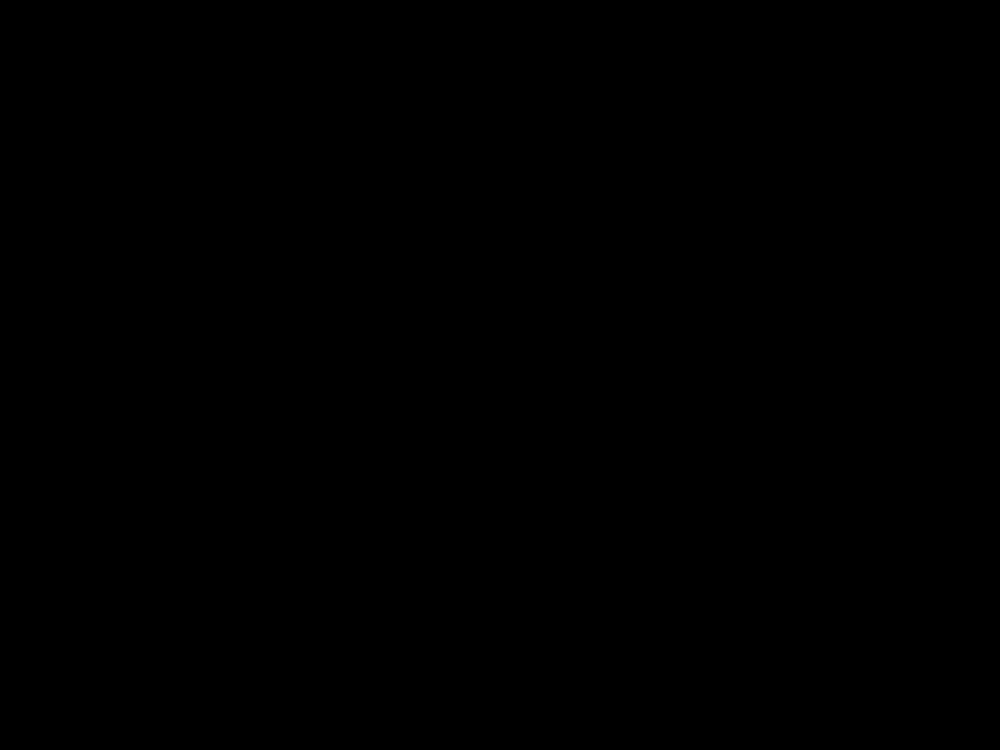
\includegraphics[width=30mm]{images/placeholder.png}}}%
%   \qquad
%   \subfloat[caption 2]{{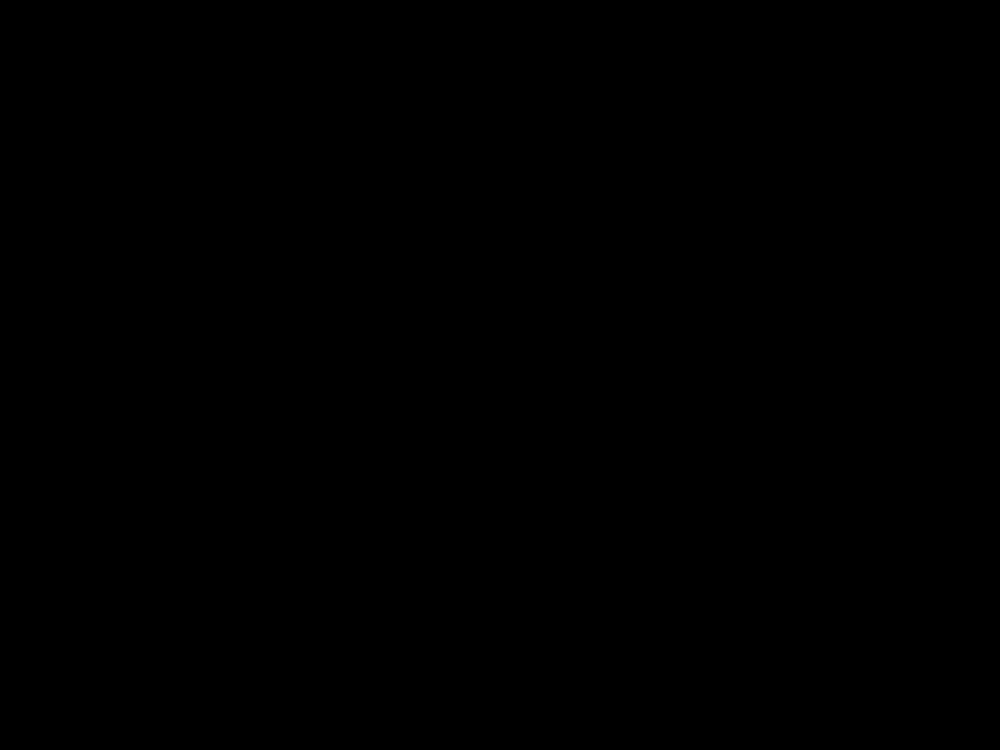
\includegraphics[width=30mm]{images/placeholder.png}}}%
%   \caption{Description}
% \end{figure}

% \begin{figure}[h]
%   \centerline{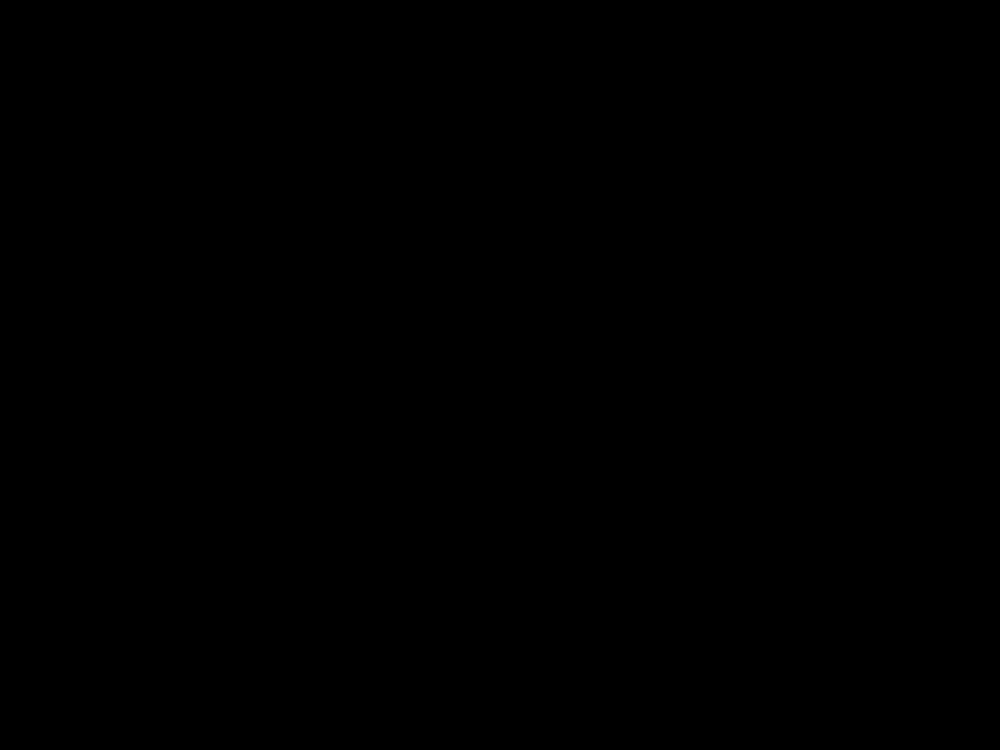
\includegraphics[width=50mm]{images/placeholder.png}}
%   \caption{Description}
% \end{figure}

%Template for a simple table 
%\begin{table}[h]
%   \caption{Description} %title of the table
%   \centering % centering table
%   \begin{tabular}{l rr} % creating three columns
%     \hline\hline %inserting double-line
%     & & \\ [0.5ex] % Insert half line vertical spacing
%     \hline % inserts single-line
%     & & \\ 
%     & & \\
%     & & \\
%     & & \\
%   \hline % inserts single-line
%   \end{tabular}
%   \label{tab:hresult}
% \end{table}
%-----------------------------------------------

\begin{document}
\setcounter{section}{0}

\section{Sequences and limits}


\subsection{Definition of a sequence}
A sequence can be thought of as a list of numbers or as a type of function which maps an input from $\N$ to $\R$. Sequences can be defined either explicitly, or recursively. An explicit definition is a sequence which is defined at any point as some function of $n$. A recursive definition is a sequence in which the value for $a_n$ is defined in terms of $a_{n-1}$\footnote{or when $n+1$ is defined in terms of $n$, it's the same}. Some sequences can be defined only explicitly. Others can be defined exclusivly with recursion. Some sequences both work.
\begin{itemize}
  \item Explicit: $a_n = f(n)$
  \item Recursively: $a_n = g(a_{n-1})$ or $a_n = g(a_{n-1}, a_{n-2})$. Note that recursive definitions require initial values to be computed.
\end{itemize}
Sequences can be denoted in multiple ways, for example:
\begin{equation*}
  a_1,a_2,a_3,\cdots,a_n,\cdots
\end{equation*}
This is more compactly denoted as:
\begin{equation*}
  \{ a_n\} \quad \text{or} \quad \{ a_n \}_{n=1}^\infty
\end{equation*}
An example of a sequence is as follows:
\begin{equation*}
  \{a_0, a_1, a_2, a_3, \cdots \} = \{1, 2, 4, 8, 16, \cdots \}
\end{equation*}
Defining this sequence explicitly gives:
\begin{equation*}
  a_n = 2^n
\end{equation*}
defining it recursively gives:
\begin{equation*}
  a_n = 2a_{n-1}, \; a_0 = 1
\end{equation*}
Another example:
\begin{equation*}
  \{a_0, a_1, a_2, a_3, \cdots \} = \{2, 0, 2, 0, 2, \cdots \}
\end{equation*}
This sequence can be given with the following explicit form:
\begin{equation*}
  a_n = 1 - (-1)^n
\end{equation*}


\subsection{Limits and sequences}
Some sequences blow up to infinity with sufficiently large choice of n, other converge to 1 single value. We can use a limit to find whether a sequence is convergent, divergent or neither. The limit of sequence can be formally defined as such:\\
A sequence $\{ a_n \}$ has a limit $L$ if for every $\epsilon > 0$ there is a corresponding integer value $N \in \N$ such that $n\geq N$ and $|a_n - L| < \epsilon$.\\
What this means informaly that the limit of a sequences denoted as $\lim_{n \to \infty} a_n = L$ exists if we can get arbitrarily close to $L$ for a sufficiently large $n$. If the limit exists a sequence is convergent.\\
Let $\lim_{n \to \infty} a_n = L \in \R$, $\lim_{n \to \infty} b_n = M \in \R$, $c \in \R$. Some algebraic rules for working with limits are:
\begin{itemize}
  \item $\lim_{n \to \infty} c\cdot a_n = c \cdot L$
  \item $\lim_{n \to \infty} a_n \pm b_n = L \pm M$
  \item $\lim_{n \to \infty} a_n \cdot b_n = L \cdot M$
  \item $\lim_{n \to \infty} \frac{a_n}{b_n} = \frac{L}{M}$, iff $M \neq 0$
\end{itemize}
Furthermore if $\lim_{x\to \infty} f(x) = L$ and $f(n) = a_n$ when $n \in \N$, then $\lim_{n \to \infty} a_n = L$.


\subsection{Evaluating limits}
Evaluating limits can often give undefined forms such as $\infty \pm \infty$, $\frac{0}{0}$ and $\frac{\infty}{\infty}$. In these cases usual procedure is to divide every term by the highest polynomial power. For example:
\begin{align*}
  \lim_{x\to\infty} \sqrt{2 + 6x + 4x^2} &= \lim_{x \to \infty} \sqrt{\frac{2}{x^2} + \frac{6x}{x^2} + \frac{4x^2}{x^2}}\\
  &= \lim_{x\to\infty} \sqrt{0 + 0 + 4} = 2
\end{align*}
In some cases the limit can be difficult to actually calculate. In such cases the squeeze theorem can be a helpfull tool. The theorem states that: if $a_n \leq b_n \leq c_n$ for $n \geq N$ and $\lim_{n\to \infty} a_n = \lim_{n\to \infty} c_n = L$, then the $\lim_{n\to \infty} b_n = L$. This is best illustrated with an example.
We want to find out whether the following sequence converges or diverges:
\begin{equation*}
  \{a_n\} = \left\{ \frac{\sin(n)}{n} \right\}
\end{equation*}
Recall that $-1 \leq \sin(n) \leq 1$. Therefore:
\begin{equation*}
  \frac{-1}{n} \leq \frac{\sin(n)}{n} \leq \frac{1}{n}, \; n>0
\end{equation*} 
If we then choose $\{ b_n\} = \left\{ \frac{-1}{n} \right\}$ and  $\{ c_n\} = \left\{ \frac{1}{n} \right\}$ we find that:
\begin{equation*}
  \lim_{n\to\infty} \{b_n\} = \lim_{n\to\infty} \{c_n\} = 0
\end{equation*}
This means that by Squeeze theorem the limit of $\{a_n\}$ must also be equal to 0. This is visualized in figure 1.1.
\begin{figure}[h]
  \centerline{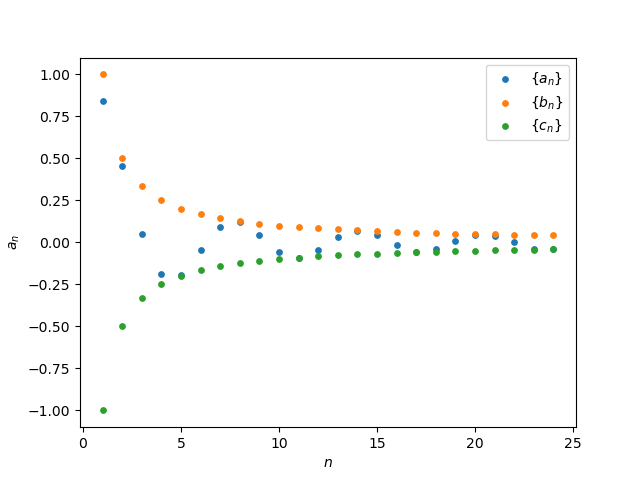
\includegraphics[width=100mm]{images/Squeeze_Theorem.png}}
  \caption{Squeeze theorem visualized. $\{ b_n\}$ converges to $0$, $\{ c_n\}$ also converges to $0$, and since $\{ a_n\}$ is in between both of them it must also converge to $0$. $\{ a_n\} = \frac{\sin(n)}{n}$, $\{ b_n\} = \frac{-1}{n}$ and $\{ a_n\} = \frac{1}{n}$.}
\end{figure}
Evaluating limits of sequences defined recursively rather then explicitly is a bit different. let $\{ a_n \}_{n=1}^\infty$ be defined as follows:
\begin{equation*}
  a_{n+1} = g(a_n)
\end{equation*}
For a continuous function $g: \R \to \R$. If $\lim_{n\to \infty} a_n = L$ exists then $L = g(L)$.


\subsection{L' Hospital's rule}
In some cases the following can happen when eveluating limits:
\begin{equation*}
  \lim_{x\to a} \frac{f(x)}{g(x)} = \frac{0}{0} \quad \text{or} \quad \lim_{x\to a} \frac{f(x)}{g(x)} = \frac{\pm \infty}{\pm \infty}
\end{equation*}
Where either $a \in \R$ or $a = \pm \infty$. L' Hospital'sis another way to evelaute these limits and states that:
\begin{equation*}
  \lim_{x \to a}\frac{f(x)}{g(x)} = \lim_{x \to a} \frac{f'(x)}{g'(x)} = L
\end{equation*}
An example of the application of this is eveluating the limit of $\frac{\sin(x)}{x}$.
\begin{align*}
  \lim_{x\to 0} \frac{\sin(x)}{x} &= \lim_{x\to 0} \frac{\cos(x)}{1} \\
                                  &= \frac{1}{1} = 1
\end{align*}


\subsection{Monotome and bounded sequences}
Sequences can either be increasing or decreasing. A sequence is defined to be increasing if for all $n \geq 1$ $a_n < a_{n+1}$. Logically a sequence is decreasing if for all $n \geq 1$ $a_n > a_{n+1}$. Sometimes the terms not-decreasing and not-increasing are also as less strict versions of increasing and decreasing. Even weaker still the term eventually increasing/decreasing is sometimes used for sequences which will increase/decrease first and start decreasing/increasing again for a sufficiently large $n$. Furthermore a sequence is monotome if it is either increasing or decreasing. Thus we end up with the following list:
\begin{itemize}
  \item $\{ a_n \}$ is increasing if $a_n < a_{n+1}$ for all $n \geq 1$
  \item $\{ a_n \}$ is not dencreasing if $a_n \leq a_{n+1}$ for all $n \geq 1$
  \item $\{ a_n \}$ is decreasing if $a_n > a_{n+1}$ for all $n \geq 1$
  \item $\{ a_n \}$ is not increasing if $a_n \geq a_{n+1}$ for all $n \geq 1$
  \item $\{ a_n \}$ is monotome if it is either increasing or decreasing
\end{itemize}
Sequences can be bounded. The bound refers to some maximum or minimum value which the sequence will not exceed. A set is bounded if it is both upper and lower bounded.
\begin{itemize}
  \item $\{ a_n\}_{n=1}^\infty$ is upper bounded if a value $M$ exists such that $a_n \leq M$ for all $n\geq 1$
  \item $\{ a_n\}_{n=1}^\infty$ is upper bounded if a value $m$ exists such that $a_n \geq M$ for all $n\geq 1$
  \item $\{ a_n\}_{n=1}^\infty$ is bounded if it is both upper and lower bounded
\end{itemize}
When a set is both bounded and monotome it will always be convergent.

\end{document}